\section{Analysis: RMSE vs Spike Rate for Constant Driving Force}




We analyse the network described by equations (\ref{eq:rotated_voltage_dynamics}) and (\ref{eq:rho_dot} for the case of a constant (in time) driving force $c(\xi) = k \mathcal{U}_j$. First we derive explicit expressions for the network estimate, then we compute the resulting RMSE for various driving strengths $k$.\\
\begin{enumerate}
\item Let 
\begin{align*}
A &= -\begin{bmatrix}  
1 & 0 \\
0 & 1
\end{bmatrix},\notag \\
\notag \\
B &= \begin{bmatrix}  
1 & 0 \\
0 & 1
\end{bmatrix}, \notag \\
\notag \\
c(\xi) &= k \mathcal{U}_1 \\
\notag \\
d\xi &= 10^{-4},\notag \\
\notag \\
N &= 4,\notag \\
\notag \\
x(0) &= \begin{bmatrix} \frac{1}{2} & 0 \end{bmatrix}.\notag 
\end{align*}

With the given initial conditions, $v_j = 0$ for $j \neq 1$ for all $\xi$. The dynamics simplify to 
\begin{equation*}
\label{eq:simple_voltage_dynamics_constant_driving}
\dot{v_1} = \Lambda_1 v_1 + (\Lambda_1 + 1)\rho_1 + k - \Omega_1.
\end{equation*}

\item We assume that the decoding matrix D is chosen such that $S_1 = 1$. Because A is the negative identity matrix, it is also clear that $\Lambda_1 = -1$. The preceding equation simplifies to  
\begin{equation}
\label{eq:simple_voltage_dynamics_constant_driving}
\dot{v_1} = -v_1 + k - \Omega_1,
\end{equation}
which is a form of the well-known Leaky Integrate-and-Fire (LIF) model. Assuming a spike has occurred at $v_{th} = \frac{1}{2}$, the voltage has just been reset so that $v_1(0) = -\frac{1}{2}$. Until the next spike, the neuron's trajectory is integrated as 
\begin{align*}
v(\xi) =  k - e^{-\xi} (k + \frac{1}{2}).
\end{align*}

Neglecting any spike reset, the voltage will asymptotically approach $v_1=k$. Thus for any spiking to occur, we must have $k \geq v_{th}$. In this case, the time required to reach a spike threshold $v_{th}$ is 
\begin{align*}
v_{th} &=  k - e^{-\xi_{spike}} (k + \frac{1}{2})
\\
\\
\implies 
e^{-\xi_{spike}} &=  \frac{k - v_{th}}{k + \frac{1}{2}}
\\
\\
&= \frac{1 - \frac{v_{th}}{k}} {1 + \frac{1}{2k}}\\
\\
 \implies
 \xi_{spike} &= - ln
 \left(
 \frac{1 - \frac{v_{th}}{k}} {1 + \frac{1}{2k}}
  \right)
 \\
 \\
 \implies 
 \frac{1}{\xi_{spike}} &= - \frac{1}{ 
 ln
 \left(
 \frac{1 - \frac{v_{th}}{k}} {1 + \frac{1}{2k}}
  \right)
 } \\
 \\
 &=   \frac{1}{ 
 ln \left(
  1 + \frac{1}{2k}
  \right) 
  -
 ln
 \left(
 1 - \frac{v_{th}}{k}\right),
 }
\end{align*}
which determines the frequency  at which the LIF neuron spikes.  Denote this frequency as a function of driving strength $k$ by $\phi(k)$:
\begin{align}
\label{eq:freq_vs_driving_strength_const}
\phi(k) \overset{\Delta}{=}  \frac{1}{ 
 ln \left(
  1 + \frac{1}{2k}
  \right) 
  -
 ln
 \left(
 1 - \frac{v_{th}}{k}\right)
 }.
\end{align}
\\

\begin{figure}
\centering
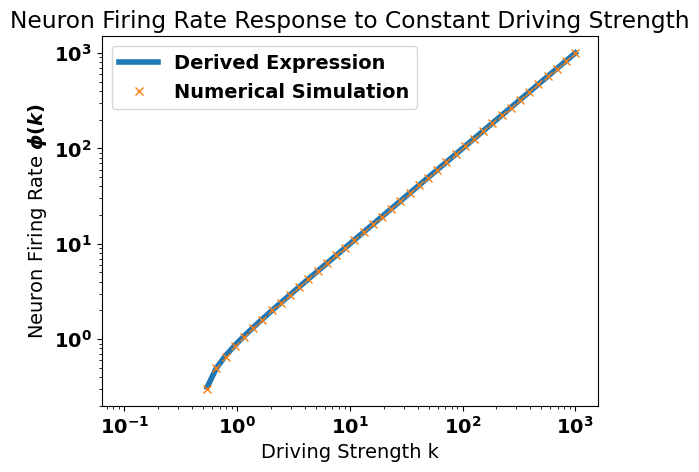
\includegraphics[width=\linewidth]{figures/phi_vs_k_const_driving.png}
\caption{A log-log plot of equation (\ref{eq:freq_vs_driving_strength_const}) alongside the rates measured from numerical simulations. The simulation parameters are described at the beginning of this section, with the decoder matrix $D$ chosen to be the first d rows of the N x N identity matrix. This ensures the singular values $S_j = 1$ as assumed in the derivation.   The rate was measured as the number of spike resets divided by the duration of the simulation. }\label{fig:spike_rate_vs_k_const_driving}
\end{figure}

The network will encode the constant driving force by spiking at a fixed rate determined by equation $(\ref{eq:freq_vs_driving_strength_const})$. Figure (\ref{fig:spike_rate_vs_k_const_driving}) shows a plot of equation (\ref{eq:freq_vs_driving_strength_const}) along with numerically computed spike rates for a simulated network driven with constant drive strength $k$.  Similar to membrane voltage, the resulting PSC and readout dynamics are reduced to one neuron periodically spiking:
\begin{align*}
\dot{\rho_1} &= -\rho_1 + \Omega_1 \\ 
\\
\implies 
\dot{\hat{x}} &= - \mathcal{U}_1 \rho_1 + \mathcal{U}_1 \Omega_1\\
\\ 
&= - \hat{x} + \mathcal{U}_1 \Omega_1. 
\end{align*}



\item The spike train $\Omega_1$ is a periodic sequence of impulses spaced in time by $\frac{1}{\phi(k)}$. Hence $\Omega_1(\xi) = \sum_{l=0}^{\infty} \delta \left(\xi - \frac{l}{\phi(k)}\right).$
The network estimate therefore has dynamics
\begin{align}
\label{eq:estimation_dynamics_const_driving}
\dot{\hat{x}} &= -\hat{x}  + \mathcal{U}_1 \sum_{l=0}^{\infty} \delta \left(\xi - \frac{l}{\phi(k)}\right).
\end{align}

The target dynamical system is
\begin{align*}
\dot{x} = - x + k 
 \mathcal{U}_1 \\
 x(0) = \begin{bmatrix} \frac{1}{2} & 0 \end{bmatrix},
\end{align*}
which has a stable fixed point at
\begin{align}
\label{eq:steady_state_dynamics_const_driving}
x = k \mathcal{U}_1.
\end{align}

\item Equation (\ref{eq:estimation_dynamics_const_driving}) implies that the network estimate $\hat{x}$ will decay until the first spike $\xi_1^1$ occurs:
\begin{align*}
\hat{x}(\xi) = x(0) e^{-\xi}, \hspace{4mm} 0 \leq \xi < \frac{1}{\phi(k)}.
\end{align*}


 At this instant, the vector $\mathcal{U}_1$ is added to the network estimate.
 \begin{align*}
 \hat{x}( \frac{1}{\phi(k)}) =  x(0) e^{- \frac{1}{\phi(k)}} + \mathcal{U}_1.
 \end{align*}
 
Decay again occurs until the next spike
\begin{align*}
\hat{x}(\xi) &= \hat{x}(\frac{1}{\phi(k)}) e^{-(\xi - \frac{1}{\phi(k)})}, \\
\\
&= \left( x(0) e^{- \frac{1}{\phi(k)}} + \mathcal{U}_1 \right)e^{-(\xi - \frac{1}{\phi(k)})} , \hspace{4mm} 
\frac{1}{\phi(k)} \leq \xi < \frac{2}{\phi(k)}\\
\\
\implies
\hat{x}(\frac{2}{\phi(k)}) &= \left( x(0) e^{- \frac{1}{\phi(k)}} + \mathcal{U}_1 \right) e^{-(\frac{1}{\phi(k)})} + \mathcal{U}_1\\
\\
&= x(0)
e^{-\frac{2}{\phi(k)}} + \mathcal{U}_1 e^{-\frac{1}{\phi(k)}} 
+ \mathcal{U}_1.
\end{align*}

The third spike more clearly shows the recursive behavior
\begin{align*}
\hat{x}(\frac{3}{\phi(k)}) &= \left[x(0)
e^{-\frac{2}{\phi(k)}} + \mathcal{U}_1 e^{-\frac{1}{\phi(k)}} 
+ \mathcal{U}_1\right] e^{-\frac{1}{\phi(k)}} + \mathcal{U}_1\\
\\
&= x(0) e^{-\frac{3}{\phi(k)}} + \mathcal{U}_1 e^{-\frac{2}{\phi(k)}} 
+ \mathcal{U}_1 e^{-\frac{1}{\phi(k)}} + \mathcal{U}_1
\end{align*}
Let us consider the $n^{th}$ spike sufficiently far from $\xi=0$ such that the transient term $x(0)e^{-\frac{n}{\phi(k)}}$ can be neglected. This leads to the expression

\begin{align*}
\hat{x}(\frac{n}{\phi(k)}) &= \sum_{l=0}^{n-1} \mathcal{U}_1 e^{- \frac{l}{\phi(k)}}  \\
\\
&= \mathcal{U}_1 \frac
{ 1 - e^{-\frac{n}{\phi(k)}}  }
{ 1 - e^{-\frac{1}{\phi(k)}}  }.
\end{align*}

For sufficiently large $n$, this converges to 
\begin{align}
\label{eq:steady_state_estimate_const_driving}
\hat{x}(\xi_1^n) = \frac{\mathcal{U}_1}{1 - e^{-\frac{1}{\phi(k)}}}.
\end{align}


\begin{figure}[h]
\centering
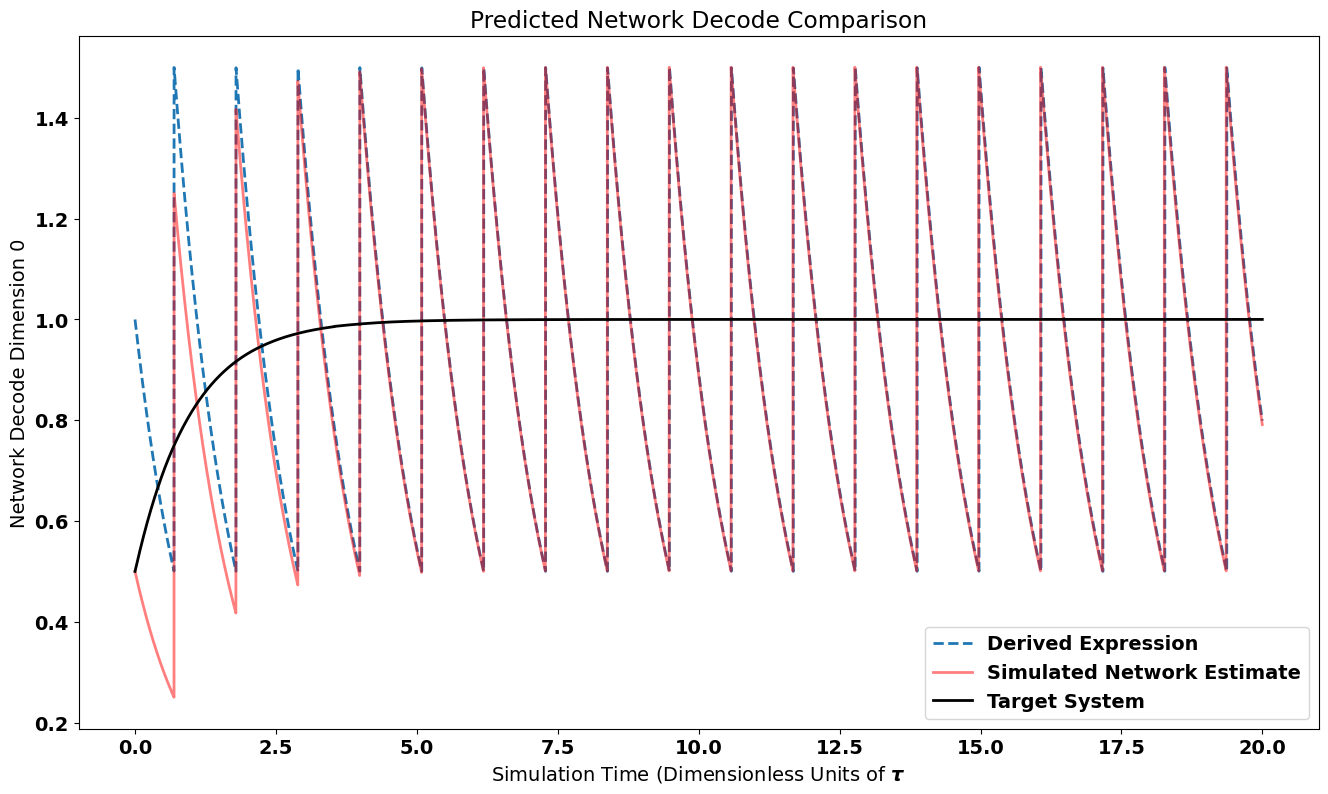
\includegraphics[width=\linewidth]{figures/network_decode_long_term_estimate_const_driving.png}
\caption{Comparison of the derived long-term network estimate equation (\ref{eq:const_driving_network_estimate_explicit_expression_long_term}) to numerical simulation. Parameters are the same as the previous figure, with $k = 1$.}
\label{fig:const_driving_convergence_to_derived_spike_readout}
\end{figure}

\item The preceding argument states that after a transient interval, the network estimate at any spike time $\xi_1^n$ is given by equation (\ref{eq:steady_state_estimate_const_driving}). As shown in figure (\ref{fig:const_driving_convergence_to_derived_spike_readout}), this convergence occurs after roughly 5 spikes for the case $k = 1$. 


We know from equation (\ref{eq:estimation_dynamics_const_driving}) that the estimate will decay exponentially from this value over an interval $\frac{1}{\phi(k)}$ until a spike returns it returns to the initial value. Thus the network estimate between two consecutive spikes is given by 
\begin{align*}
\hat{x}(\xi) = \frac{\mathcal{U}_1}{1 - e^{-\frac{1}{\phi(k)}}} e^{-(\xi - \xi_1^n)}, \hspace{4mm} 0 \leq \xi - \xi_1^n  < \frac{1}{\phi(k)}.
\end{align*}

Combine this expression with equation (\ref{eq:steady_state_estimate_const_driving}), we have an explicit expression for the long-term behavior of the network estimate given by 

\begin{equation}
\label{eq:const_driving_network_estimate_explicit_expression_long_term}
\hat{x}(\xi) =
\frac{\mathcal{U}_1}{1 - e^{-\frac{1}{\phi(k)}}} e^{- (\xi - \xi_1^1) \mod{\frac{1}{\phi(k)}}},
\end{equation} 
where $x \mod{y}$ denotes the fractional remainder of $x$ after division by $y$. 

\clearpage

\item Assume the true system dynamics have settled to their fixed point $x = k \mathcal{U}_1$. From equation (\ref{eq:const_driving_network_estimate_explicit_expression_long_term}) the network estimate $\hat{x}$ and therefore error $e = x - \hat{x}$ is a periodic function of $\xi$ with period $\frac{1}{\phi(k)}$. The RMSE over any integer number of spike periods is easily calculated from the RMSE over a single spike period. 

We compute the per-spike RMSE of the error signal  $e$ by 
\begin{equation}
\label{eq:per_spike_rmse_def}
RMSE_{spike} \overset{\Delta}{=} \sqrt{\phi(k) \int_{0}^{\frac{1}{\phi(k)}} \!  ||e(\tau)||^2 \, \, \mathrm{d}\tau}.
\end{equation}

The integrand $||e(\tau)||^2$ simplifies to 

\begin{align*}
e^T e &= (x - \hat{x})^T (x - \hat{x}) \\
\\
&= x^T x - 2 x^T \hat{x} + \hat{x}^T \hat{x} \\
\\
&= k^2 \, \mathcal{U}_1 ^T \mathcal{U}_1 - 2 k \, \,  \mathcal{U}_1^T \mathcal{U}_1 \frac{e^{- \tau}}{1 - e^{-\frac{1}{\phi(k)}}} 
+ 
\mathcal{U}_1^T \mathcal{U}_1  \left(\frac{e^{- \tau}}{1 - e^{-\frac{1}{\phi(k)}}} \right)^2\\
\\
&= k^2 - \frac{ 2 k \, e^{- \tau}}{1 - e^{-\frac{1}{\phi(k)}}} 
+ 
\frac{e^{- 2\tau}}{\left(1 - e^{-\frac{1}{\phi(k)}}\right)^2}.
\end{align*}

Therefore the integral is

\begin{align*}
\phi(k)\int_{0}^{\frac{1}{\phi(k)}} \!  ||e(\tau)||^2 \, \, \mathrm{d}\tau &= 
\phi(k)\int_{0}^{\frac{1}{\phi(k)}} \!  
k^2 - \frac{ 2 k \, e^{- \tau}}{1 - e^{-\frac{1}{\phi(k)}}} 
+ 
\frac{e^{- 2\tau}}{\left(1 - e^{-\frac{1}{\phi(k)}}\right)^2}
\, \, \mathrm{d}\tau\\
\\
&= k^2 + \phi(k) \frac{2 k }{1 - e^{-\frac{1}{\phi(k)}}} \left( e^{- \frac{1}{\phi(k)}} - 1 \right) 
- \phi(k) \frac{1}{ 2 \, \left(1 - e^{-\frac{1}{\phi(k)}}\right)^2} 
\left( e^{ -  \frac{2}{\phi(k)}} - 1 \right) \\
\\
&= k^2  + \phi(k) \left[ \frac{1 - e^{-\frac{2}{\phi(k)}}}{2 \left(1 - e^{-\frac{1}{\phi(k)}} \right)^2}  -2 k \right]  .
\end{align*}


The per-spike RMSE of the network estimate as a function of drive strength $k$ is therefore
\begin{equation}
\label{eq:per_spike_rmse_const_driving_k}
RMSE_{spike}(k) =
\sqrt{k^2  + \phi(k) \left[ \frac{1 - e^{-\frac{2}{\phi(k)}}}{2 \left(1 - e^{-\frac{1}{\phi(k)}} \right)^2}  -2 k \right] }.
\end{equation}

To write the RMSE explicitly as a function of firing rate $\phi(k)$, we invert equation (\ref{eq:freq_vs_driving_strength_const}) to obtain
\begin{align*}
k(\phi)&=  \frac{ v_{th} + \frac{e^{-\frac{1}{\phi}}}{2}}{1 - e^{-\frac{1}{\phi}}}.
\end{align*}

Substitute this for k to obtain

\begin{align}
\label{eq:per_spike_rmse_const_driving_phi}
RMSE_{spike}(\phi) &=
\sqrt{k(\phi)^2  + \phi \left[ \frac{1 - e^{-\frac{2}{\phi}}}{2 \left(1 - e^{-\frac{1}{\phi}} \right)^2}  -2 k(\phi) \right] } \notag
%
\\ 
\\
%
&= 
\sqrt{
     \left(
		     \frac
			{
			v_{th} + \frac{e^{- \frac{1}{\phi}      }}{2}
			}
			{
			1 - e^{-\frac{1}{\phi}   }
			}
      \right)^2
  +
   \phi \left[ \frac{1 - e^{-\frac{2}{\phi}}}{2 \left(1 - e^{-\frac{1}{\phi}} \right)^2}  
   -2 \, 
			    \frac
			{
			v_{th} + \frac{e^{-\frac{1}{\phi}   }}{2}
			}
			{
			1 - e^{-\frac{1}{\phi}   }
			}
     \right]
     } \notag.
\end{align}

Equations (\ref{eq:per_spike_rmse_const_driving_k}) and (\ref{eq:per_spike_rmse_const_driving_phi}) are plotted in figure (\ref{fig:const_driving_per_spike_rmse_vs_phi_k}). Note that the drive strength varies the amplitude of the target system's steady state. Thus we have derived the the network performance over its dynamic range of representable state space. 



\begin{figure}[h]
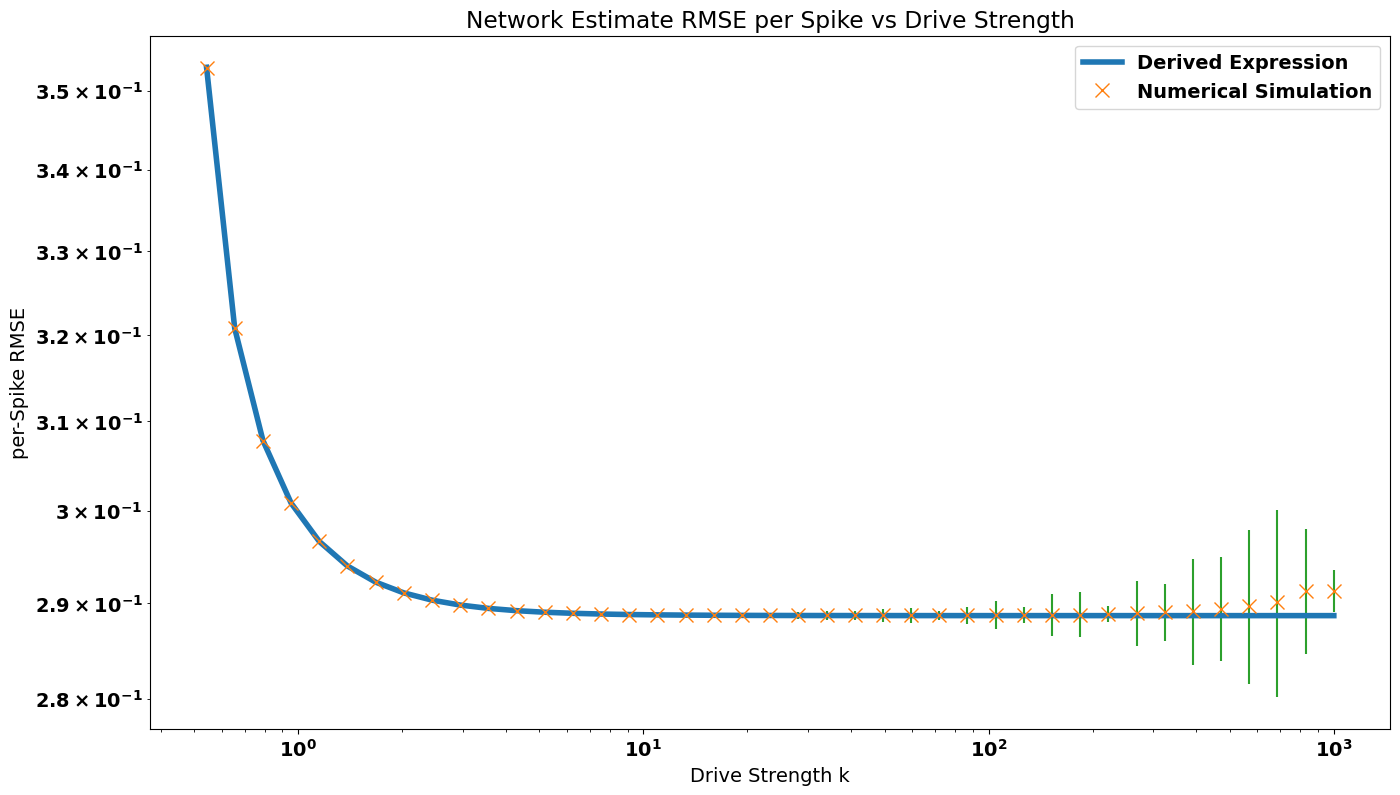
\includegraphics[width=\linewidth]{figures/rmse_sp_vs_k_const_driving.png}
\centering
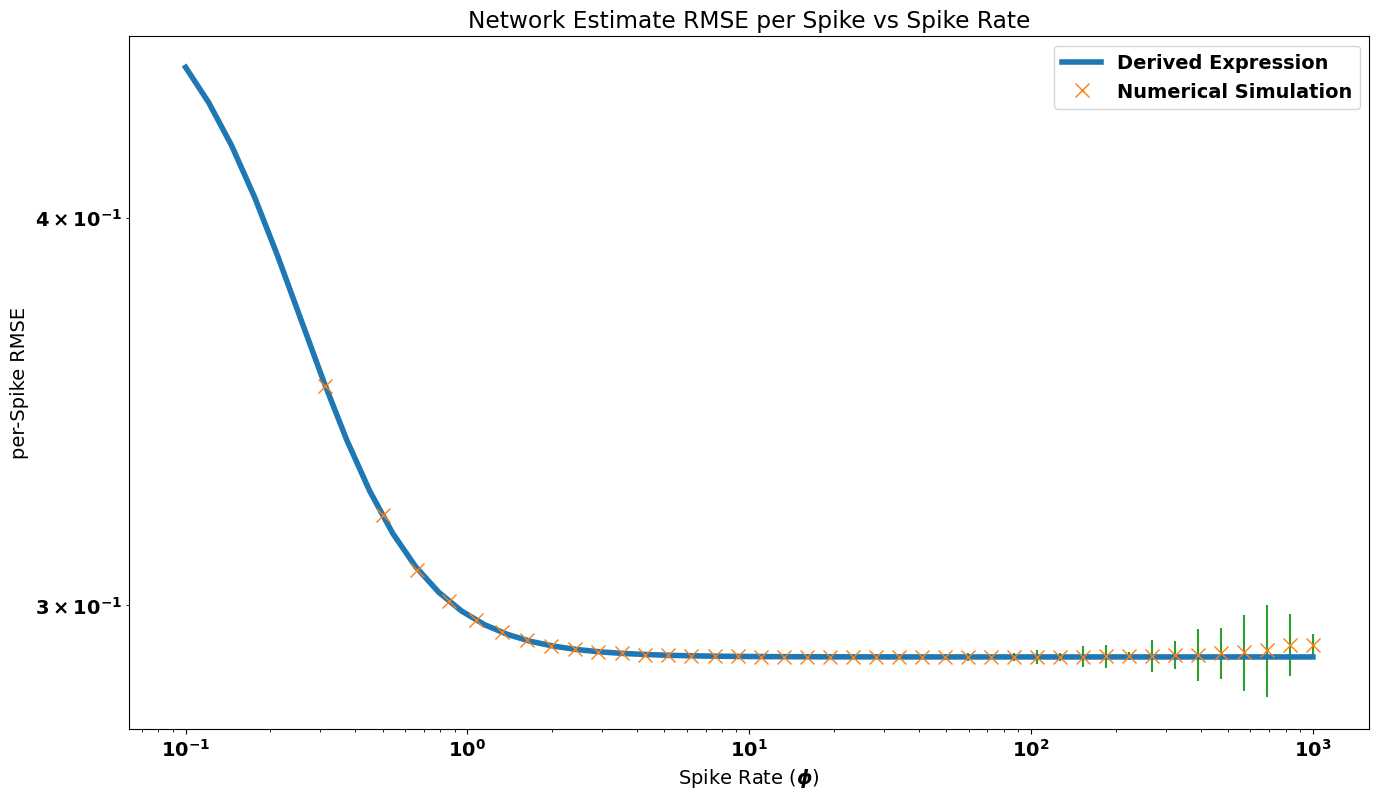
\includegraphics[width=\linewidth]{figures/rmse_sp_vs_phi_const_driving.png}
\caption{\textbf{\textit{Top:}} A log-log plot of equation (\ref{eq:per_spike_rmse_const_driving_k}). \textbf{\textit{Bottom:}} A log-log plot of equation (\ref{eq:per_spike_rmse_const_driving_phi}). \textbf{\textit{Both:}} Each simulated data point is the RMSE averaged over all inter-spike intervals in a simulation of length $T = 80 \tau_s$ at a constant (in time) drive strength. Between simulations, the spike rates were varied by sweeping drive strength. Green vertical lines towards the larger values are +/- 1 standard deviation. The spike rates $\hat{\phi}$ were computed numerically via dividing the number of spikes in a simulation by the simulation duration. The RMSE between two adjacent spikes was computed by numerical integration as a discrete sum: $\hat{RMSE} = \sqrt{\hat{\phi} \sum_{\tau \text{ between spikes }} e(\xi)^T e(\xi) \, \, d\xi }$. The increase in standard deviation is due to finite approximation error from numerical integration.}
\label{fig:const_driving_per_spike_rmse_vs_phi_k}
\end{figure}
\end{enumerate}
